\documentclass[conference]{IEEEtran}

\usepackage{cite}
% IEEEtran's default typewriter face (Courier / pcrr7t) is not in TeX Live
% Basic; Computer Modern tt keeps \texttt usable without extra font packages.
\renewcommand{\ttdefault}{cmtt}
\usepackage{amsmath,amssymb,bm}
\usepackage{graphicx}
\usepackage{booktabs}
\usepackage{tikz}
\usepackage{url}
\usepackage{xcolor}
\usepackage{balance}
\usetikzlibrary{arrows.meta,positioning,calc,fit}

\hyphenation{Whisper Jacobian decoder-only verbal-izable}

\begin{document}

\title{A Decoder-Only Jacobian Lens for Speech-to-Text Models}

\author{
\IEEEauthorblockN{Januda Lelwala, Anas Hussaindeen, Chandupa Ambepitiya, and Dewmike Amarasinghe}
\IEEEauthorblockA{Department of Computer Science and Engineering\\
University of Moratuwa, Sri Lanka}
}

\maketitle

\begin{abstract}
Encoder--decoder speech recognizers such as Whisper fuse acoustic evidence into a decoder residual stream that is then unembedded as tokens. We ask whether the Jacobian lens---introduced to identify verbalizable representations in language models---transfers to this decoder. A natural first attempt, a pooled encoder-to-decoder transport, destroys the causal \((t,t')\) structure of the map and yields scores without logit semantics. We instead fit one averaged, position-resolved Jacobian per decoder layer,
\(J_\ell=\mathbb{E}_{t,\,t'\ge t}[\partial h_{\mathrm{final},t'}/\partial h_{\ell,t}]\),
estimated with Hutchinson probes, and read out with the model's own output projection:
\(\mathrm{lens}(h)=\mathrm{softmax}(E\,J_\ell h)\).
The resulting \((\text{position}\times\text{layer})\) grid is implemented in ECHO, an audio interpretability workbench. Qualitative readings recover crystallization depth, an audio-only workspace at the start-of-transcript token, language-prior versus acoustic evidence, and precursor signatures of hallucination loops.
\end{abstract}

\begin{IEEEkeywords}
speech recognition, mechanistic interpretability, Jacobian lens, Whisper, encoder--decoder Transformers
\end{IEEEkeywords}

\section{Introduction}

Automatic speech recognition (ASR) models such as Whisper~\cite{radford2023whisper} are now accurate enough that \emph{how} they transcribe matters as much as \emph{what} they transcribe. Hallucinated repetitions under silence, homophone substitutions, and early cutoffs are familiar failure modes, yet the internal state that produces the next token is rarely inspected in vocabulary space.

A parallel question has just been posed for language models. Gurnee et~al.~\cite{gurnee2026workspace} introduce the \emph{Jacobian lens}: an average causal map from a layer's residual stream to the final pre-logit state, read out with the model's own unembedding. The tokens that this readout ranks are the representations the model is \emph{poised to verbalize}. In LLMs those representations occupy a mid-depth band with the functional hallmarks of a global workspace.

Speech-to-text models look, at first glance, like a hard case for the same construction. The residual stream is split across two components. Acoustic computation lives in an encoder that is never unembedded; verbalization lives in a decoder that attends to the encoder through cross-attention~\cite{vaswani2017attention}. The question is which stream the lens should read.

This short paper answers: the decoder, and only the decoder. We port the LLM Jacobian-lens estimator to Whisper's decoder residual stream, fit it with Hutchinson probes~\cite{hutchinson1989trace} so that the encoder can sit outside the autograd graph, and ship the result as a first-class tool in ECHO, a Learning Interpretability Tool for audio models~\cite{tenney2020lit}. Along the way we record why the obvious alternative---a pooled transport from encoder blocks into the decoder---is the wrong object.

Contributions:
\begin{itemize}
\item A decoder-only J-lens for seq2seq ASR that matches the LLM construction: same-space maps, causal averaging over \(t'\ge t\), readout \(\mathrm{softmax}(EJh)\).
\item A failure analysis of pooled encoder transports (destroyed alignment, off-manifold unembedding, scores without probability semantics).
\item An implementation in ECHO, with a \((\text{position}\times\text{layer})\) visualization and a linear closed-form test, plus qualitative readings of Whisper-base.
\end{itemize}

\section{Related Work}

\textbf{Lenses on language models.}
The logit lens~\cite{nostalgebraist2020logitlens} applies the unembedding to intermediate residuals (identity transport). The tuned lens~\cite{belrose2023tuned} learns an affine map to the final layer. The Jacobian lens~\cite{gurnee2026workspace} is neither: it is the \emph{average derivative} of the true residual-to-final map, not a regression onto final states. We copy that estimator, not the LLM causal suite (write, hold, ablate), which we do not claim to have reproduced.

\textbf{Encoder--decoder interpretation.}
DecoderLens~\cite{langedijk2024decoderlens} skips encoder layers into a frozen decoder to ask what the encoder has computed. Complementary: they interpret the encoder \emph{through} the decoder; we interpret the decoder \emph{with} its own Jacobian. Linear probes~\cite{alain2017probes,hewitt2019structural,belinkov2022probing} diagnose linearly available features but are not causal maps onto the model's unembedding.

\textbf{Speech tooling.}
ECHO is the audio analogue of LIT~\cite{tenney2020lit}: attention, saliency, embeddings, and perturbations on Whisper and wav2vec~2.0~\cite{baevski2020wav2vec2}. Attention says where the decoder looked in the audio; saliency says which waveform regions moved a scalar. Neither says what the decoder is poised to say. CTC models have no decoder residual to unembed and are excluded.

\section{Method}

\subsection{Substrate}

Whisper is an encoder--decoder Transformer. For a clip, the encoder emits a length-1500 acoustic sequence (30\,s of log-Mel, stride~2). The decoder, at each transcript position \(t\), attends causally to the prefix and, via cross-attention, to all 1500 encoder frames, then unembeds with a tied projection \(E\). On Whisper-base, both stacks have width \(d=512\) and six blocks; the Hugging Face decoder reports seven residual streams (embedding output plus six blocks). The fit target is the model's last hidden state, the post-final-LayerNorm tensor that \(E\) consumes. We write \(h_{\ell,t}\in\mathbb{R}^d\) for the residual at lens-layer \(\ell\) and position \(t\), and \(h_{\mathrm{final},t'}\) for that target.

The encoder is a substrate, not a workspace. It never sees \(E\). Gradients for the lens therefore never enter it: one frozen forward provides cross-attention keys and values.

\subsection{Estimator}

Following~\cite{gurnee2026workspace}, the lens at layer \(\ell\) is the expected causal Jacobian
\begin{equation}
J_\ell \;=\;
\mathbb{E}_{t,\,t'\ge t,\,\text{clip}}
\!\left[
\frac{\partial h_{\mathrm{final},t'}}{\partial h_{\ell,t}}
\right]
\in\mathbb{R}^{d\times d}.
\label{eq:J}
\end{equation}
The expectation is over source positions, future positions allowed by the causal mask, and a corpus of teacher-forced transcripts. There is no optimizer and no learned baseline: the model is frozen in evaluation mode, and \(J_\ell\) is \emph{measured}.

Exact Jacobians are unnecessary. A Rademacher probe \(r\in\{\pm 1\}^d\) and one vector--Jacobian product of \(\sum_{t'}\langle h_{\mathrm{final},t'},r\rangle\) yield, at every source \(t\) simultaneously, \(\sum_{t'\ge t}J_\ell(t\!\to\! t')^\top r\), because the causal mask zeroes \(t>t'\)~\cite{hutchinson1989trace}. Averaging \(\mathrm{outer}(r,\sum_t g_t)\) over probes and clips, and dividing by the triangular count \(T(T+1)/2\), estimates~\eqref{eq:J}. The encoder sits outside this graph.

\subsection{Readout}

At apply time the decoder actually runs: greedy generation, or a provided reference transcript, produces the positions; a teacher-forced pass collects \(h_{\ell,t}\). Each cell is
\begin{equation}
\mathrm{lens}(h_{\ell,t})
\;=\;
\operatorname{softmax}\bigl(E\,J_\ell h_{\ell,t}\bigr).
\label{eq:lens}
\end{equation}
Whisper's final LayerNorm is inside the decoder, so it is absorbed into \(J_\ell\); we do not apply an extra RMS-norm. Scores sit on the model's logit scale. Top-\(k\) (default \(k=5\)) is a \emph{ranking} of verbalizable content, not a phrase, and the softmax is for display, not calibrated confidence.

The readout axis is transcript position, not audio time. Which encoder frame supports a token remains a cross-attention question.

\subsection{Why encoder transports fail}

An earlier design fitted a global map from the mean-pooled encoder state to the mean-pooled decoder state and applied it to 0.3\,s encoder buckets (Table~\ref{tab:redesign}). That object is not~\eqref{eq:J}. Differentiating \emph{after} pooling erases \((t,t')\) alignment; the linearization is around whole-clip means but is applied locally; the unembedding is used off-manifold with the constant term dropped, so scores have no probability semantics. CTC support came for free (the encoder is the only stream) and disappeared with the redesign, correctly: a CTC head never verbalizes through a decoder workspace.

\begin{table}[!t]
\caption{Encoder transport versus decoder-only lens.}
\label{tab:redesign}
\centering
\setlength{\tabcolsep}{3pt}
\begin{tabular}{@{}p{0.12\columnwidth}p{0.38\columnwidth}p{0.38\columnwidth}@{}}
\toprule
 & Pooled encoder transport & Decoder-only J-lens \\
\midrule
Source & mean of 1500 encoder frames & residual \(h_{\ell,t}\) \\
Target & mean of \(T\) decoder positions & \(h_{\mathrm{final},t'}\), \(t'\ge t\) \\
Spaces & encoder \(\to\) decoder & decoder \(\to\) decoder \\
Readout & \((h-\bar h)J^\top E^\top\) & \(\mathrm{softmax}(EJh)\) \\
Units & 0.3\,s buckets & decoder tokens \\
\bottomrule
\end{tabular}
\end{table}

\section{Implementation}

The lens is a job in ECHO (Fig.~\ref{fig:arch}). Fit writes a format-v2 artifact: architecture ``decoder'', method Hutchinson-decoder-VJP, one square \(d\times d\) matrix per recorded decoder state, bound to a model revision. Apply refuses a mismatch. Only seq2seq ASR adapters expose the architecture; wav2vec~2.0 returns none.

On Whisper-base the grid has seven rows (embedding output plus six blocks). Unit tests recover the closed form \(J=2M/(T+1)\) for a linear decoder with causal triangular averaging, and check apply against an independent \((Jh)E^\top\) recomputation.

\begin{figure}[!t]
\centering
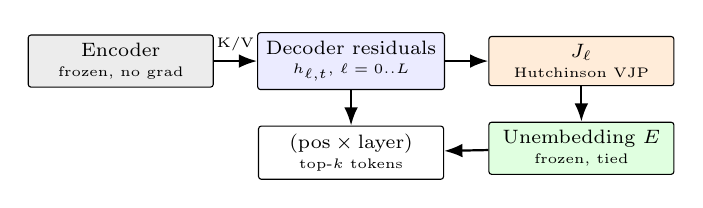
\begin{tikzpicture}[
  font=\scriptsize,
  box/.style={draw, rounded corners=1pt, align=center, inner sep=3pt, minimum height=0.62cm},
  arr/.style={-{Latex}, thick}
]
\node[box, fill=gray!15, minimum width=2.35cm] (enc) {Encoder\\[-1pt]{\tiny frozen, no grad}};
\node[box, fill=blue!8, minimum width=2.35cm, right=0.55cm of enc] (dec) {Decoder residuals\\[-1pt]{\tiny \(h_{\ell,t}\), \(\ell=0..L\)}};
\node[box, fill=orange!15, minimum width=2.35cm, right=0.55cm of dec] (j) {\(J_\ell\)\\[-1pt]{\tiny Hutchinson VJP}};
\node[box, fill=green!12, minimum width=2.35cm, below=0.45cm of j] (e) {Unembedding \(E\)\\[-1pt]{\tiny frozen, tied}};
\node[box, minimum width=2.35cm, below=0.45cm of dec] (grid) {\((\text{pos}\times\text{layer})\)\\[-1pt]{\tiny top-\(k\) tokens}};
\draw[arr] (enc) -- node[above, font=\tiny] {K/V} (dec);
\draw[arr] (dec) -- (j);
\draw[arr] (j) -- (e);
\draw[arr] (e) -- (grid);
\draw[arr] (dec) -- (grid);
\end{tikzpicture}
\caption{ECHO decoder-only J-lens. The encoder supplies cross-attention keys and values and is never differentiated. Each decoder layer has its own \(J_\ell\); readout uses the model's \(E\).}
\label{fig:arch}
\end{figure}

\section{What the grid shows}

The following readings are observational, from Whisper-base in the ECHO lab. They are hypotheses to measure, not census results. Layer \(0\) is the embedding output; layer \(6\) is the last decoder block.

\textbf{Crystallization depth.}
A column (one position, all layers) typically moves from frequent-token rankings in the early rows, through syntactic candidates, to the spoken word in the upper-middle band. The row of convergence is a candidate for the depth at which acoustics enter the verbal decision. Columns that never converge mark transcription against the model's internal preference.

\textbf{Start-of-transcript as audio-only workspace.}
At the start-of-transcript token the decoder has consumed no transcript tokens. Everything in the residual arrived through cross-attention. The top tokens at this position are an acoustic gist of the clip---likely first words, Whisper's silence convention, or background-speech artifacts---the closest available reading of ``what the audio alone put into the workspace.''

\textbf{Prior versus evidence.}
When mid and late layers agree on a collocation, the token is language-model driven. When mid layers stay generic and the top rows flip to an unusual word, the token came from the audio. Sweeping that disagreement is a per-word prior-versus-evidence map.

\textbf{Hallucination precursors.}
Under silence, Whisper's repetition loop is often ranked highly in mid layers \emph{before} generation commits. The grid is a leading indicator, not only a post-hoc explanation.

\textbf{Ambiguity and endpoints.}
A wide top-\(k\) spread at a position (their/there/they're) flags under-determined acoustics. Near the end of speech, readouts drift toward end-of-text, punctuation, or trained closers such as ``thank you''; premature stop-direction while speech continues is an early-cutoff signature.

These patterns are the speech analogue of the LLM observation that early-layer readouts are noise and that a mid-depth band carries verbalizable content~\cite{gurnee2026workspace}. Confirming a workspace \emph{range} with a layer-wise top-1 agreement curve is left as future work.

\section{Limitations}

The map is a first-order average: rankings are more trustworthy than absolute scores, and a position far from the fit distribution will be misread. Because \(J_\ell\) averages over pairs, the lens cannot name the supporting audio frame. Fit targets are teacher-forced, so \(J\) reflects ``given this prefix,'' not free-running generation. Hutchinson probes (we default to four) leave residual estimation noise. Frequent-token geometry biases rankings. The artifact is model-revision bound. Write-mode interventions (steer, ablate, patch) from~\cite{gurnee2026workspace} are not implemented. We report no large-scale census.

\section{Conclusion}

The Jacobian lens is a statement about a residual stream that is about to be unembedded. In encoder--decoder ASR that stream is the decoder's. Fitted there, with causal averaging and the model's own \(E\), it yields a \((\text{position}\times\text{layer})\) vocabulary grid that ECHO can already show. Fitted on pooled encoder states, it yields an object that is no longer a lens. The next measurements---workspace-band statistics, multi-size Whisper, and a write mode---should be taken on the decoder construction, not the encoder one.

\section*{Acknowledgments}

We thank Dr.~Uthayasanker Thayasivam for guidance, and the ECHO-Lit group for the platform this lens ships in. The estimator follows Gurnee et~al.~\cite{gurnee2026workspace}; remaining errors are ours.

\balance
\bibliographystyle{IEEEtran}
\bibliography{references}

\end{document}
